% For easier proof-reading, use the single-column, double-spaced layout:
\documentclass{netsec2012}

% Final Paper use double-column, normal line spacing. Comment the
% above line and uncomment the following line when you are writing
% Full paper and Final paper!  
%\documentclass[cameraready]{netsec2012}

\begin{document}

%=========================================================

\title{Single-character OCR using Support Vector Machines}

\author{Olli Jarva \& Jarno Rantanen \\
        Aalto University School of Science \\
        \texttt{olli@jarva.fi} \texttt{\&} \texttt{jarno@jrw.fi}}
\maketitle

%==========================================================

\begin{abstract}

This paper describes a solution to an optical character recognition problem for bitmap characters
using Support Vector Machines with an RBF kernel, including a description of RBF parameter search
and bitmap normalization.  Classification performance of 90.8\% was achieved against a given
training set of 42152 correctly labelled samples using k-fold crossvalidation with k=20
\cite{training_set}.

\vspace{3mm}
\noindent KEYWORDS: SVM, Support Vector Machine, RBF, OCR, Character Recognition

\end{abstract}

%============================================================




% Remember that one of the objectives of the course is to teach you how to apply machine learning methods in a principled way, instead of just running some black box method on data and hoping that it will perform well. Therefore in the report it is not enough, e.g., just to explain the algorithm you implemented. Typically, the report should also include a discussion of why you selected a particular method (pros and cons), the principles of the method, validation of your approach (e.g., feature selection, model complexity selection, validation, estimation of generalization error etc.), your conclusions and other relevant issues.
% The factual content of the report must be correct and relevant. There should be sufficient amount of essential information (the length of the answer is not merit in itself). The report should give an impression that you understand what you are doing and therefore you are able to apply what you have learned in the course to machine learning problems.
% You must substantiate all of your claims. For example, you can't claim that your method will generalize well to new data if you haven't shown this, e.g., experimentally, by logical (mathematical) argumentation or by appropopriate citation. You must make a clear distinction between facts, substantiated claims and opinions (opinions being unsubstantiated claims).



\section{Data set description}

The data set against which our solution was developed consisted of a provided set of 42152
black-and-white bitmaps, depicting hand-written instances of characters from the English alphabet
(that is, the task was to classify the bitmaps into 26 distinct categories).  Each bitmap was given
as a 16-by-8 image, in the form of a binary vector of length 128 (meaning an array of 128 ones or
zeroes).  The vectors were delivered in a text file, with the correct label associated with each
vector.

\label{ref:datasetdescription}

As an optional extra task, we were provided with the opportunity of participating in a competition
amongst different solutions to the same classification problem.  The competition was organized by
first providing only a subset of the training data (10000 vectors), using that to train a
classifier, and then calculating an error rate against the rest of the training data (which was not
yet made available at that time).  Our participation in the competition is discussed further in
Section \ref{ref:datachallenge}.

The same data set was used for both training our classifiers, and testing them afterwards.  The data
was split using k-fold cross-validation to minimize overfitting, while making the most of the
available data.  This testing technique is discussed in further detail in Section
\ref{ref:crossvalidation}.

%Training dataset:
%
%\begin{itemize}
%\item n=42152
%\item 16 x 8 black and white bitmaps
%\item Lowercase characters, n=26 (a-z)
%\end{itemize}
%
%Testing dataset:
%
%\begin{itemize}
%\item n=10000
%\item Same format
%\end{itemize}

\section{Method selection}

There is no de-facto solution to the problem we were facing; Optical Character Recognition (OCR) is
a wide field of research with ongoing investigation into new methods.  An important factor in method
selection was simplicity - in the beginning of the project, we were not seasoned experts in OCR or
Machine Learning, so we were looking for established methods that work robustly even in the hands of
beginners.

One initial contender was Principal Component Analysis (PCA).  PCA works by reducing a
high-dimensional data set into a (hopefully) smaller set of dimensions, so that the resulting
dimensions capture most of the variance of the original space.  PCA by itself is not a complete
solution to our problem, as the data points would still have to be labelled in the dimensionally
reduced input space. \cite{ding2004k}

For this task, with or without the help of PCA, one could use basic clustering algorithms such as
k-means clustering.  k-means clustering works by identifying exactly k clusters from the input data,
without supervision.  We had pre-labelled training data at our disposal, however, so we could make
use of supervised learning methods instead. \cite{ding2004k}

\label{ref:knn}

Perhaps the simplest of all supervised machine learning methods is the k-nearest neighbor (kNN)
algorithm.  It works by assigning classes to samples by way of majority vote: for an incoming,
unlabelled sample, the k nearest neighbors are looked up (using either simple euclidian distance, or
a custom distance function).  The assigned class is decided simply by observing the class
memberships of the neighbors and choosing the most common one.  kNN is not guaranteed to work well
with high-dimensional input data, however, and would likely require at least dimensionality
reduction by PCA or other preprocessing methods. \cite{keller1985fuzzy}

In the end we chose to go with Support Vector Machines (SVM's), which were suggested by our
literature review as a relatively simple yet effective machine learning method for our type of
classification problem (OCR).  The underlying mathematics and theory of the method is beyond the
scope of this paper, and ready-made implementations are available for several common programming
languages.  Thus, an intimate understanding of the inner workings of the algorithm would not be
required, as we would only be configuring and using an SVM, and not implementing one from scratch.
SVM's are described in more detail in Section \ref{ref:svmintro} below. \cite{libsvm_guide}

Based on the performance of our solution, we have reason to believe we made a sensible choice in
using SVM's for this task.  The performance aspects are discussed further in Section
\ref{ref:datachallenge}.

%\begin{itemize}
%\item What other options were there
%\item Why we chose SVM?
%\item A nod to why we think we chose correctly
%\end{itemize}

\section{Support Vector Machines}

\label{ref:svmintro}

Support Vector Machines (SVM's) are a method for supervised machine learning, meaning they solve a
classification problem by creating a classifier function from a set of existing, labeled data
points.  This function can then be used to classify (or \emph{label}) subsequent data points
\emph{without} supervision.  In contrast to \emph{regression methods} which produce continuous
output, the output of a classifier function is always exactly one class into which the input data
point (likely) belongs.

In its most basic implementation, an SVM is trained with data labeled into exactly two separate
groups.  The resulting classifier is a \emph{binary one}, meaning it will classify subsequent input
into those same two categories.  If the input data points belong to a two-dimensional space, this
can be intuitively thought of separating the data points into two clusters.  To minimize the
potential for generalization error, the clusters should be separated by as wide a band as possible
(or in simpler terms, by a line, with as much space between the line and the nearest data points as
possible). \cite{svm_chemistry}

In mathematical terms, an SVM solves an optimization problem for pairs
$(x_i, y_i), i = 1, ..., l$ where $x_i$ is the i:th input data vector, and $y_i$ is the correct
label associated with that input:

\begin{center}
min($w,b,\xi$): $\frac{1}{2}w^Tw + C \sum_{i=1}^l\xi_i$, \\
subject to $y_i(w^T \phi(x_i) + b) \ge 1 - \xi_i, \xi_i \ge 0$,
\end{center}

where $C$ is the penalty parameter (see Section \ref{ref:kernelparamsearch} for how it is chosen),
$w$ is a support vector in the problem space, $b$ is a scalar associated with the support vector,
$\xi$ is the error term, and $\phi$ is a mapping function for the input space (the role of which is
described below). \cite{libsvm_guide,cortes1995support}

\label{ref:multiclasssvm}

SVM's generalize nicely into higher dimensional spaces.  In an n-dimensional input space, the two
classes are linearly separated by an (n-1)-dimensional hyperplane instead of a line.  They also
generalize into working with >2 classes by way of reducing the multi-class classification problem
into a set of binary classification problems.  This can be done, for example, by chaining the binary
classifiers so that the first classifies the input data as either belonging to class "A" or "other",
the second one to "B" or other, and so on. \cite{duan2005best}

The above works off the assumption that the sets being discriminated are linearly separable in the
input space.  With realistic data sets, however, this is often not the case.  To keep the sets
linearly separable (and thus the SVM approach applicable), the input space can be mapped into a much
higher-dimensional space.  The assumption is that with this added sparsity, a linearly separating
hyperplane can be found, even for problematic input data sets. \cite{svm_chemistry}

Such mappings can be achieved using what are known as \emph{kernel functions}.  Kernel functions
have special properties that, in addition to helping the linear separability, reduce the
computational load bearable.  Numerous kernel functions have been proposed in literature, and new
ones are being researched.  The performance characteristics of the functions are highly dependent on
the type of classification problem at hand, and the properties of the input space, and not all
kernels work for all problems.  There is, however, little theoretical base on how to \emph{choose} a
suitable kernel for a given data set, and thus it is in fact common to simply rely on empirical
methods and compare the performance some common kernels, choosing the one that best fits the
specific data set. \cite{svm_chemistry}

%\begin{itemize}
%\item http://www.csie.ntu.edu.tw/~cjlin/papers/guide/guide.pdf
%\item http://www.ivanciuc.org/Files/Reprint/Ivanciuc\_SVM\_CCR\_2007\_23\_291.pdf
%\item RBF kernel: $K(x_i, x_j) = exp(-\gamma || x_i - x_j ||^2), \gamma > 0$
%\item "Unique Features of SVM's and Kernel Methods" in \cite{berwick09idiots}
%\end{itemize}
%
%Optimization problem $(x_i, y_i), i = 1, ..., l$ where $x_i$ is ... (\cite{libsvm_guide}):
%
%minimize $w,b,\xi$: $\frac{1}{2}w^Tw + C \sum_{i=1}^l\xi_i$
%
%subject to $y_i(w^T \phi(x_i) + b) \ge 1 - \xi_i, \xi_i \ge 0$

\section{Kernel selection}

The Radial Basis Function (RBF) kernel is a common first-choice kernel suggested by literature
\cite{libsvm_guide,svm_chemistry}. It has several desireable properties.  Firstly, it is numerically
robust in comparison to some other kernels.  Secondly, another common alternative - the linear
kernel - is simply a special case of the RBF one.  Thirdly, and perhaps most importantly, the SVM
kernel is configured with only two parameters (as opposed to the 4 parameters of the polynomial
kernel, for example).  As the parameter search is in essence a local optimization problem, having a
2-dimensional search space makes this problem more manageable than, say, searching in 4 dimensions.
The parameter search is discussed further in Section \ref{ref:kernelparamsearch}. \cite{libsvm_guide}

We did briefly try out other kernel functions (as many are readily provided with our SVM
implementation of choice, mlpy \cite{albanese12mlpy}), but we ended up agreeing with our first
choice of RBF, as it seemed the best performer against our data set.  Also, since a much bigger part
of the effort in configuring an SVM has to do with choosing proper parameters for the kernel
function, RBF had desireable properties in that regard as well.  These are discussed further in
Section \ref{ref:kernelparamsearch}.

\section{Character preprocessing}

An SVM operates on input data represented as vectors of real numbers.  Scaling the input data is
very important with SVM's; features of the input data with large numerical ranges can easily
dominate ones with smaller ranges, even though the width of their range has no real correlation with
their importance in the actual classification problem at hand.  It is thus suggested to always scale
the data into a normalized range of [-1,1], or even [0,1]. \cite{libsvm_guide}

Much of the preprocessing for the input data in our experiment was already done for us; the image
data was nicely encoded into a set of binary vectors, so no bitmap processing was required.  Also,
since the vectors were binary, no data scaling was required.

The single preprocessing technique we opted for was basic noise reduction, by moving each image to
the bottom left corner.  That is, making sure images otherwise identical except for their padding
would still look identical to the algorithm.  We found this to increase our initial classification
performance by 0.5\%.

%\begin{itemize}
%\item Minimize noise by moving characters to bottom left corner. 0.5\% improvement
%\end{itemize}

\section{RBF kernel parameter search}

\label{ref:kernelparamsearch}

Optimal parameters for the SVM (and the kernel function) present a local optimization problem in a
2-dimensional search space.  The dimensions being explored are $\gamma$ (the RBF kernel parameter)
and $C$ (the SVM penalty parameter).  Since an exhaustive search in this space isn't possible, a
basic grid search was employed.

In the first step of the search, the space was divided into a grid of 6-by-6 (totaling 36 cells), at
each of which the classifiers were trained and the performance of the algorithm was measured.  Our
literature review (\cite{libsvm_guide} especially) suggested going for exponentially increasing
values of the parameters $\gamma$ and $C$ when doing the coarse mapping of the search space, which
seemed like a reasonable starting point.  The coarse search step covered $\gamma$ for $2^i$ with $i
= -10, -8, -6, -4, -2, 0$ and $C$ for $2^i$ with $i = -1, 1, 3, 5, 7, 9$.  Out of the explored
cells, the one at which the algorithm performed best was chosen for the next step.

In the second step, the chosen cell was further explored by fine-tuning the parameters around the
cell origin.  The search works by varying both parameters by a small percentage until the
performance converges at a local maximum.

\label{ref:crossvalidation}

The aforementioned classification performance was measured using a technique known as \emph{k-fold
cross-validation}.  In a naive implementation of classifier training, the input data would be
divided into two different sets: a training set, which is used to train the classifier, and a
validation set, that is used to measure the performance of the classifier (as both sets contain the
correct labels for data points).  This approach is not optimal, however: the classifier may suffer
from \emph{overfitting}, meaning it ends up modeling more the training set, instead of the actual
classification problem being solved.  This is due to the classifier being trained only against a
specific part of the training data, and validated against another.  How those sets are chosen (that
is, picked from the entire set of labelled data available) can greatly affect the resulting
classifier.  Should the validation data set be chosen with a bit of bad luck, for example, it may
end up containing a very specific subset of the entire data, skewing the resulting error rates.

K-fold cross-validation avoids these issues by dividing the labelled data into k-segments of equal
size, and then using each as the validation set in turn.  The rest of the segments are then used to
train the classifier being validated.  Once each segment has been validated against, the error rate
is calculated over the entire set of validations.  This both makes use of the entire data set for
training, and avoids overfitting, as all parts of the data are (at one point) used for validation.

%\begin{itemize}
%\item Initial search space 2**x for x in range(-15, 15)
%\item Select best area for next round
%\item Validate by taking final arguments and calculating error rates for +- few percent for both variables.
%\end{itemize}

\section{Classifier chaining}

During initial testing we found that certain pairs of characters were often confused by the
classifier.  As an example, the characters "i" and "l" were commonly misclassified.  To compensate
for this, we adjusted the primary classifier to treat "i" and "l" (and similar other pairs of
characters) as a single category.  Then, after the primary classification, the input data points
classified into these combined categories were sent to a second-level SVM, specifically trained to
discriminate between the two characters in the combined category.  This effectively turned our
classifier into a \emph{classifier tree}, with second-level classifiers chained to the primary SVM.

Even though this approach originally yielded classification performance improvements of a few
percent, after carefully selecting the primary classifier parameters $\gamma$ and $C$, the original
primary classifier performed better than the classifier tree.  In the end, this was both desireable
and intuitive.  It was desireable because it makes our solution simpler, and simple solutions are
easier to sanity-check.  It was intuitive (especially in retrospect) because our solution was in
fact analoguous to how multi-class SVM's are often constructed internally anyway (as discussed in
Section \ref{ref:multiclasssvm}), so it would have been unexpected had our duplication of this
construct yielded significant improvements.

%The performance
%of the classifier tree in each grid point was evaluated using k-fold cross-validation.
%Cross-validation was chosen as it provides reasonable protection against overfitting against the
%training data.

\section{Results and performance}

We were happy with the performance of our solution.  We achieved a classification performance of
90.8\% against the given training set of 42152 correctly labelled samples, as measured by k-fold
crossvalidation with k=20.  On a 2.1GHz Xeon development machine, a full run of the training and
validation phases (as the cross-validation requires several trainings and validations) for a given
combination of $\gamma$ and $C$ took approximately 6 hours (single-threaded).

\begin{table}[t]
\centering
\begin{tabular}{|r|r|r|r|}
\hline
Character & Instances & Correct (\%) & Correct \\
\hline
a &   1076 &    90.89\% &    978 \\
b &    424 &    93.40\% &    396 \\
c &    408 &    93.14\% &    380 \\
d &    562 &    88.43\% &    497 \\
e &   1192 &    93.96\% &    1120 \\
f &    198 &    80.81\% &    160 \\
g &    233 &    88.41\% &    206 \\
h &    238 &    84.03\% &    200 \\
i &    960 &    86.98\% &    835 \\
k &     92 &    90.22\% &    83 \\
l &    865 &    89.60\% &    775 \\
m &    186 &    95.16\% &    177 \\
n &    671 &    95.83\% &    643 \\
o &    457 &    97.37\% &    445 \\
p &     94 &    98.94\% &    93 \\
q &    201 &    32.34\% &    65 \\
r &    322 &    91.93\% &    296 \\
s &    304 &    92.43\% &    281 \\
t &    542 &    91.33\% &    495 \\
u &    304 &    89.14\% &    271 \\
w &    380 &    81.32\% &    309 \\
y &    188 &    84.04\% &    158 \\
z &    103 &    86.41\% &    89 \\
\hline
\end{tabular}
\caption{Per-character classification performance.  Percentages are in relation to the actual count
of the character; that is, out of all instances of the character, how many were correctly
classified.}
\label{tab:percharperformance}
\end{table}

\begin{figure}[t]
\centering
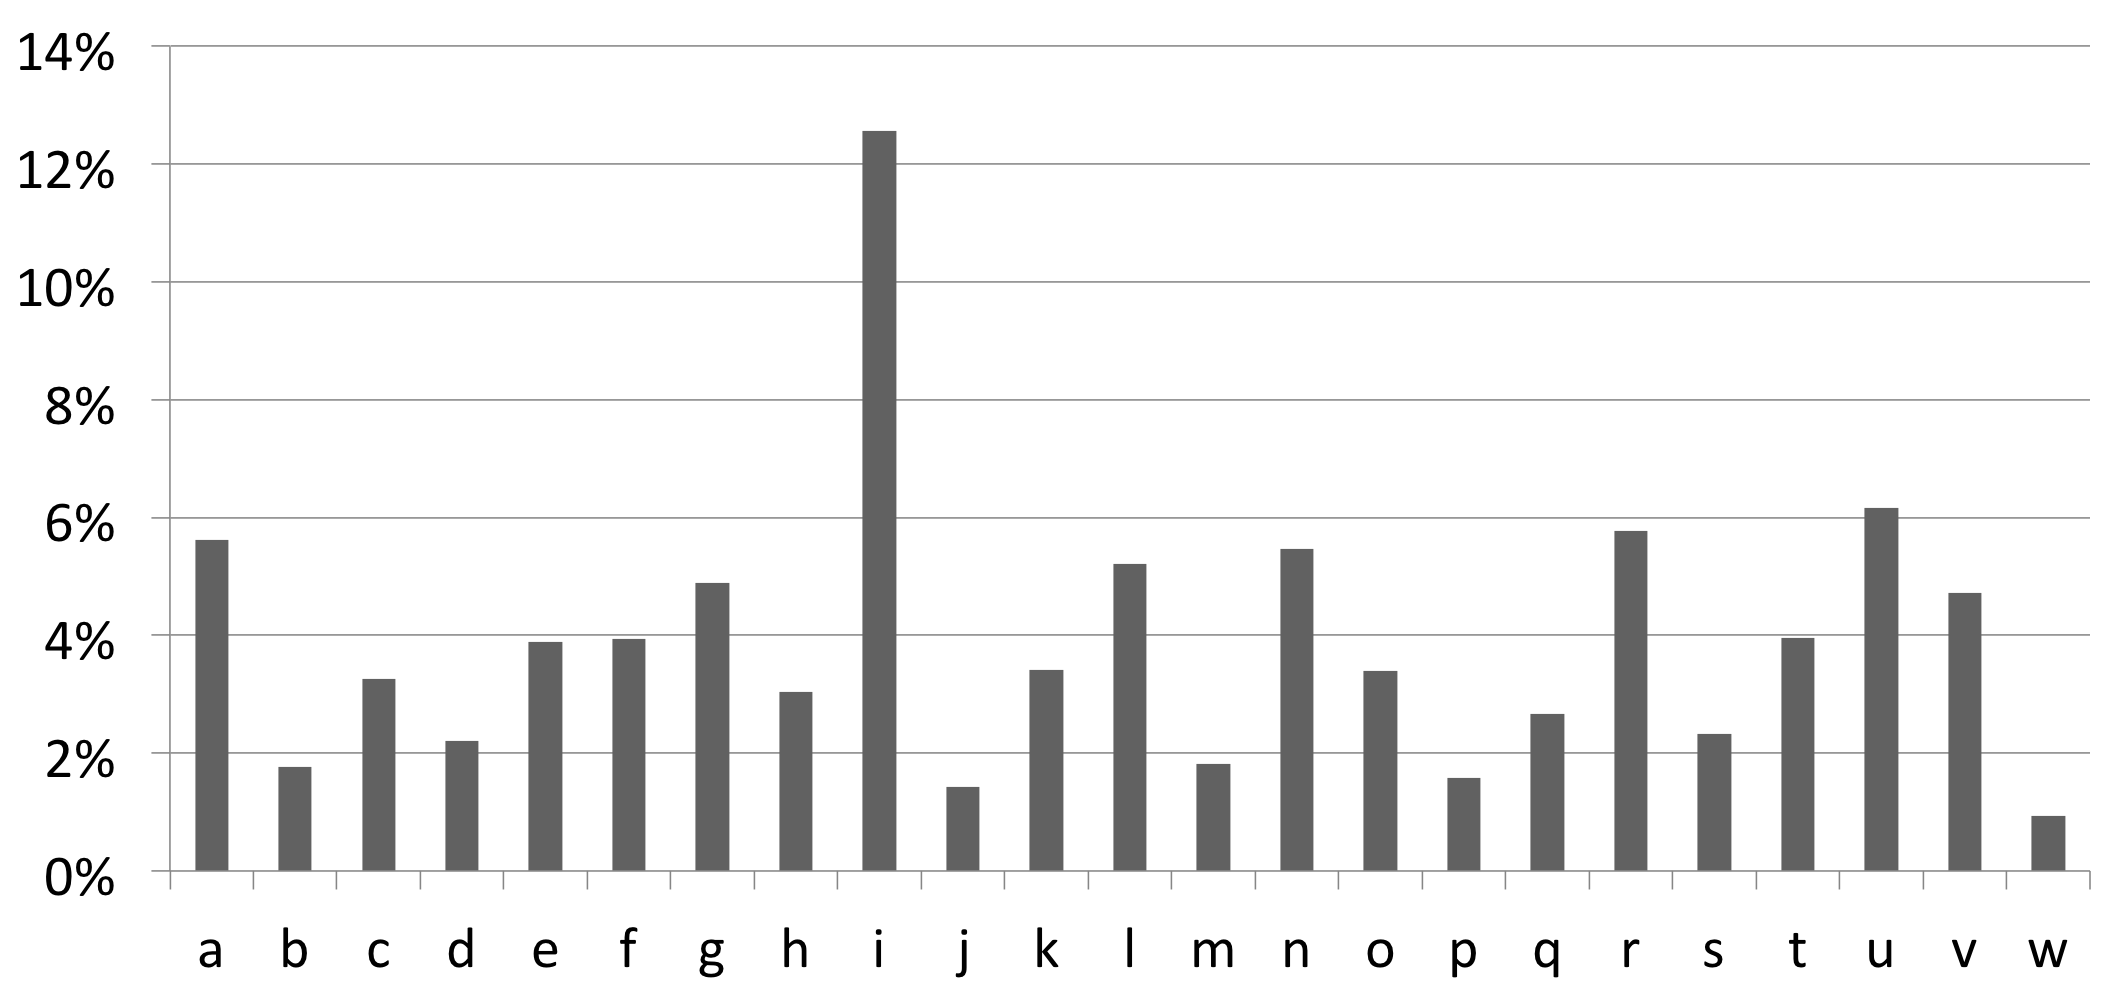
\includegraphics[width=120mm]{percharperf.png}
\caption{Per-character classification performance, visualized.  See Table
    \ref{tab:percharperformance} for the source data.}
\label{fig:percharperformance}
\end{figure}

\begin{figure}[t]
\centering
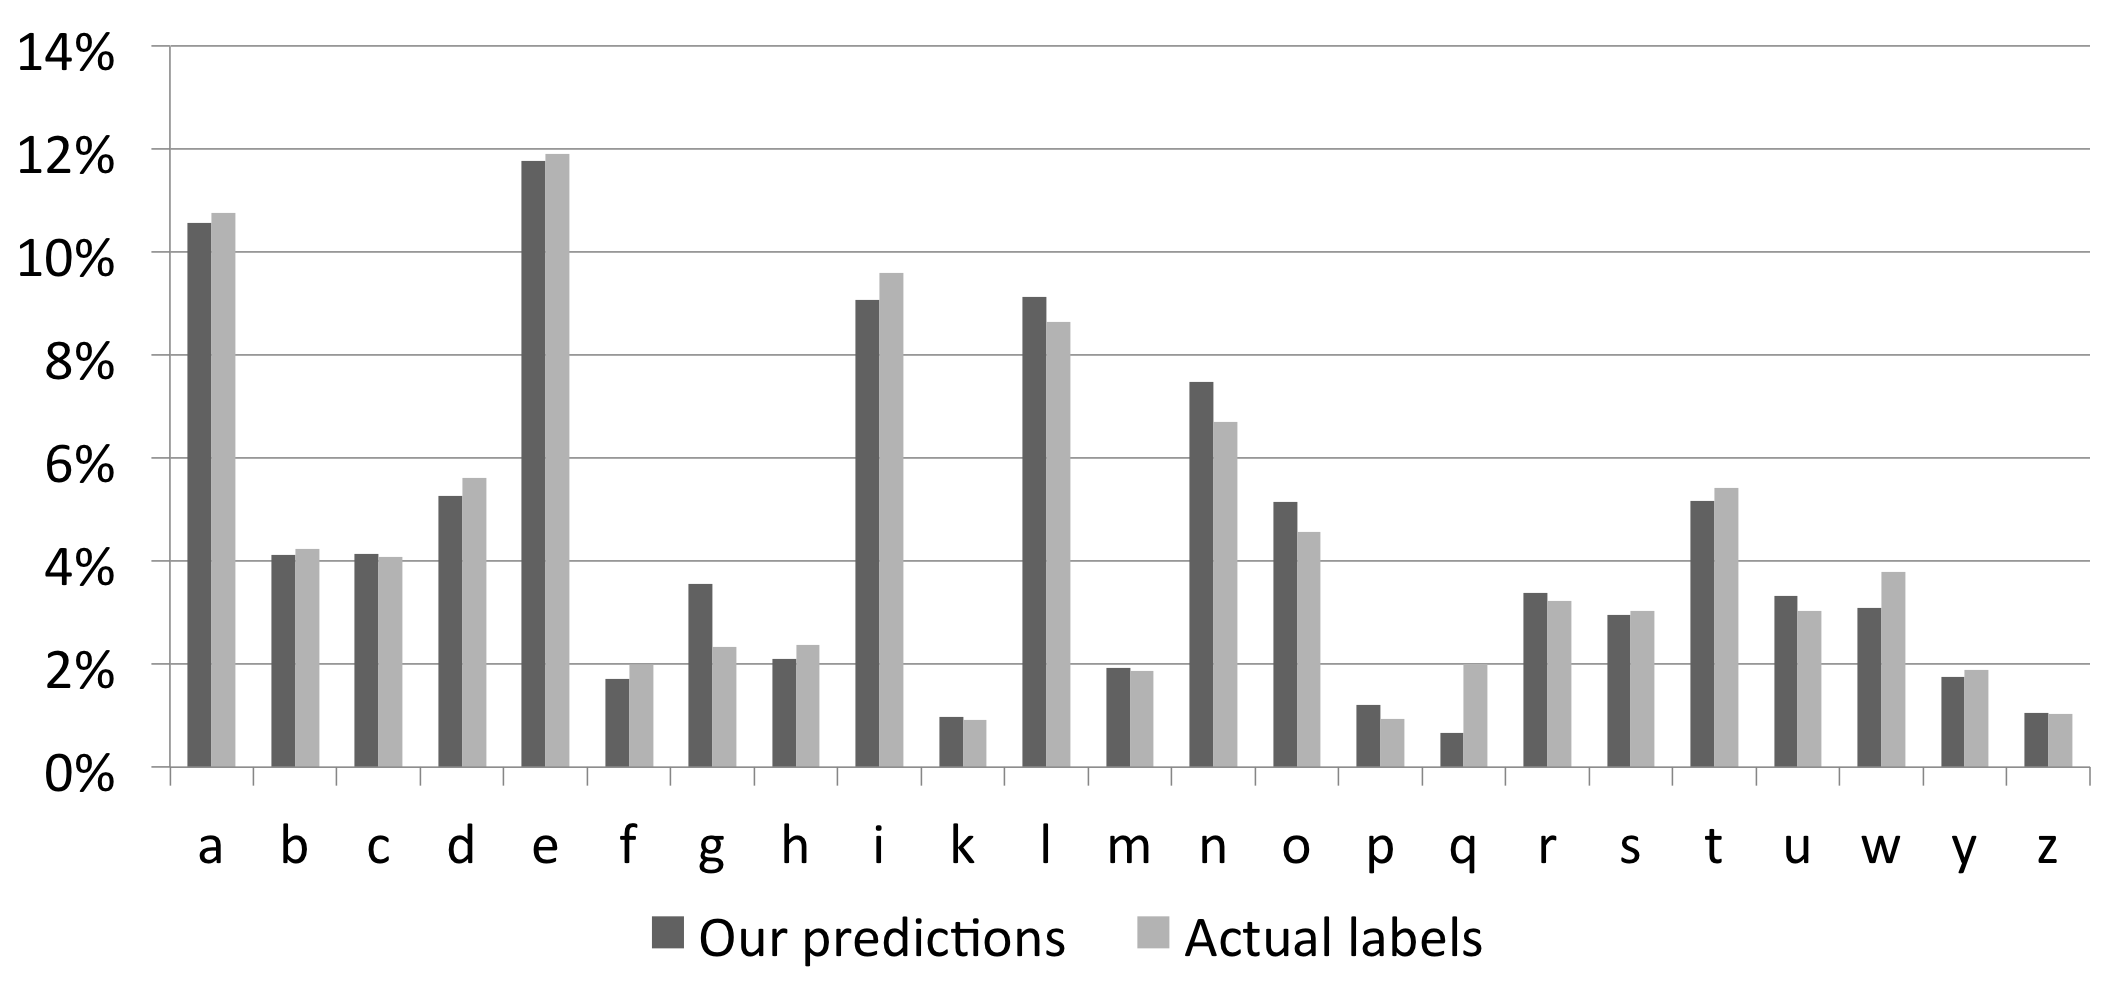
\includegraphics[width=120mm]{chardist.png}
\caption{Character distribution in the data set.  Our predictions (that is, labels assigned by our
algorithm) have been contrasted with the correctly labelled data.}
\label{fig:chardistribution}
\end{figure}

Per-character classification performance has been included in Table \ref{tab:percharperformance},
and visualized in Figure \ref{fig:percharperformance}.  The most noteworthy dip in performance is
for the character "q".  This cannot be completely explained by the per-character data alone; the
character "q" is relatively infrequent, which could explain an elevated \emph{relative}
misclassification rate, but characters such as "p" and "k" are rarer and do not suffer from such
high rates.

\begin{figure}[t]
\centering
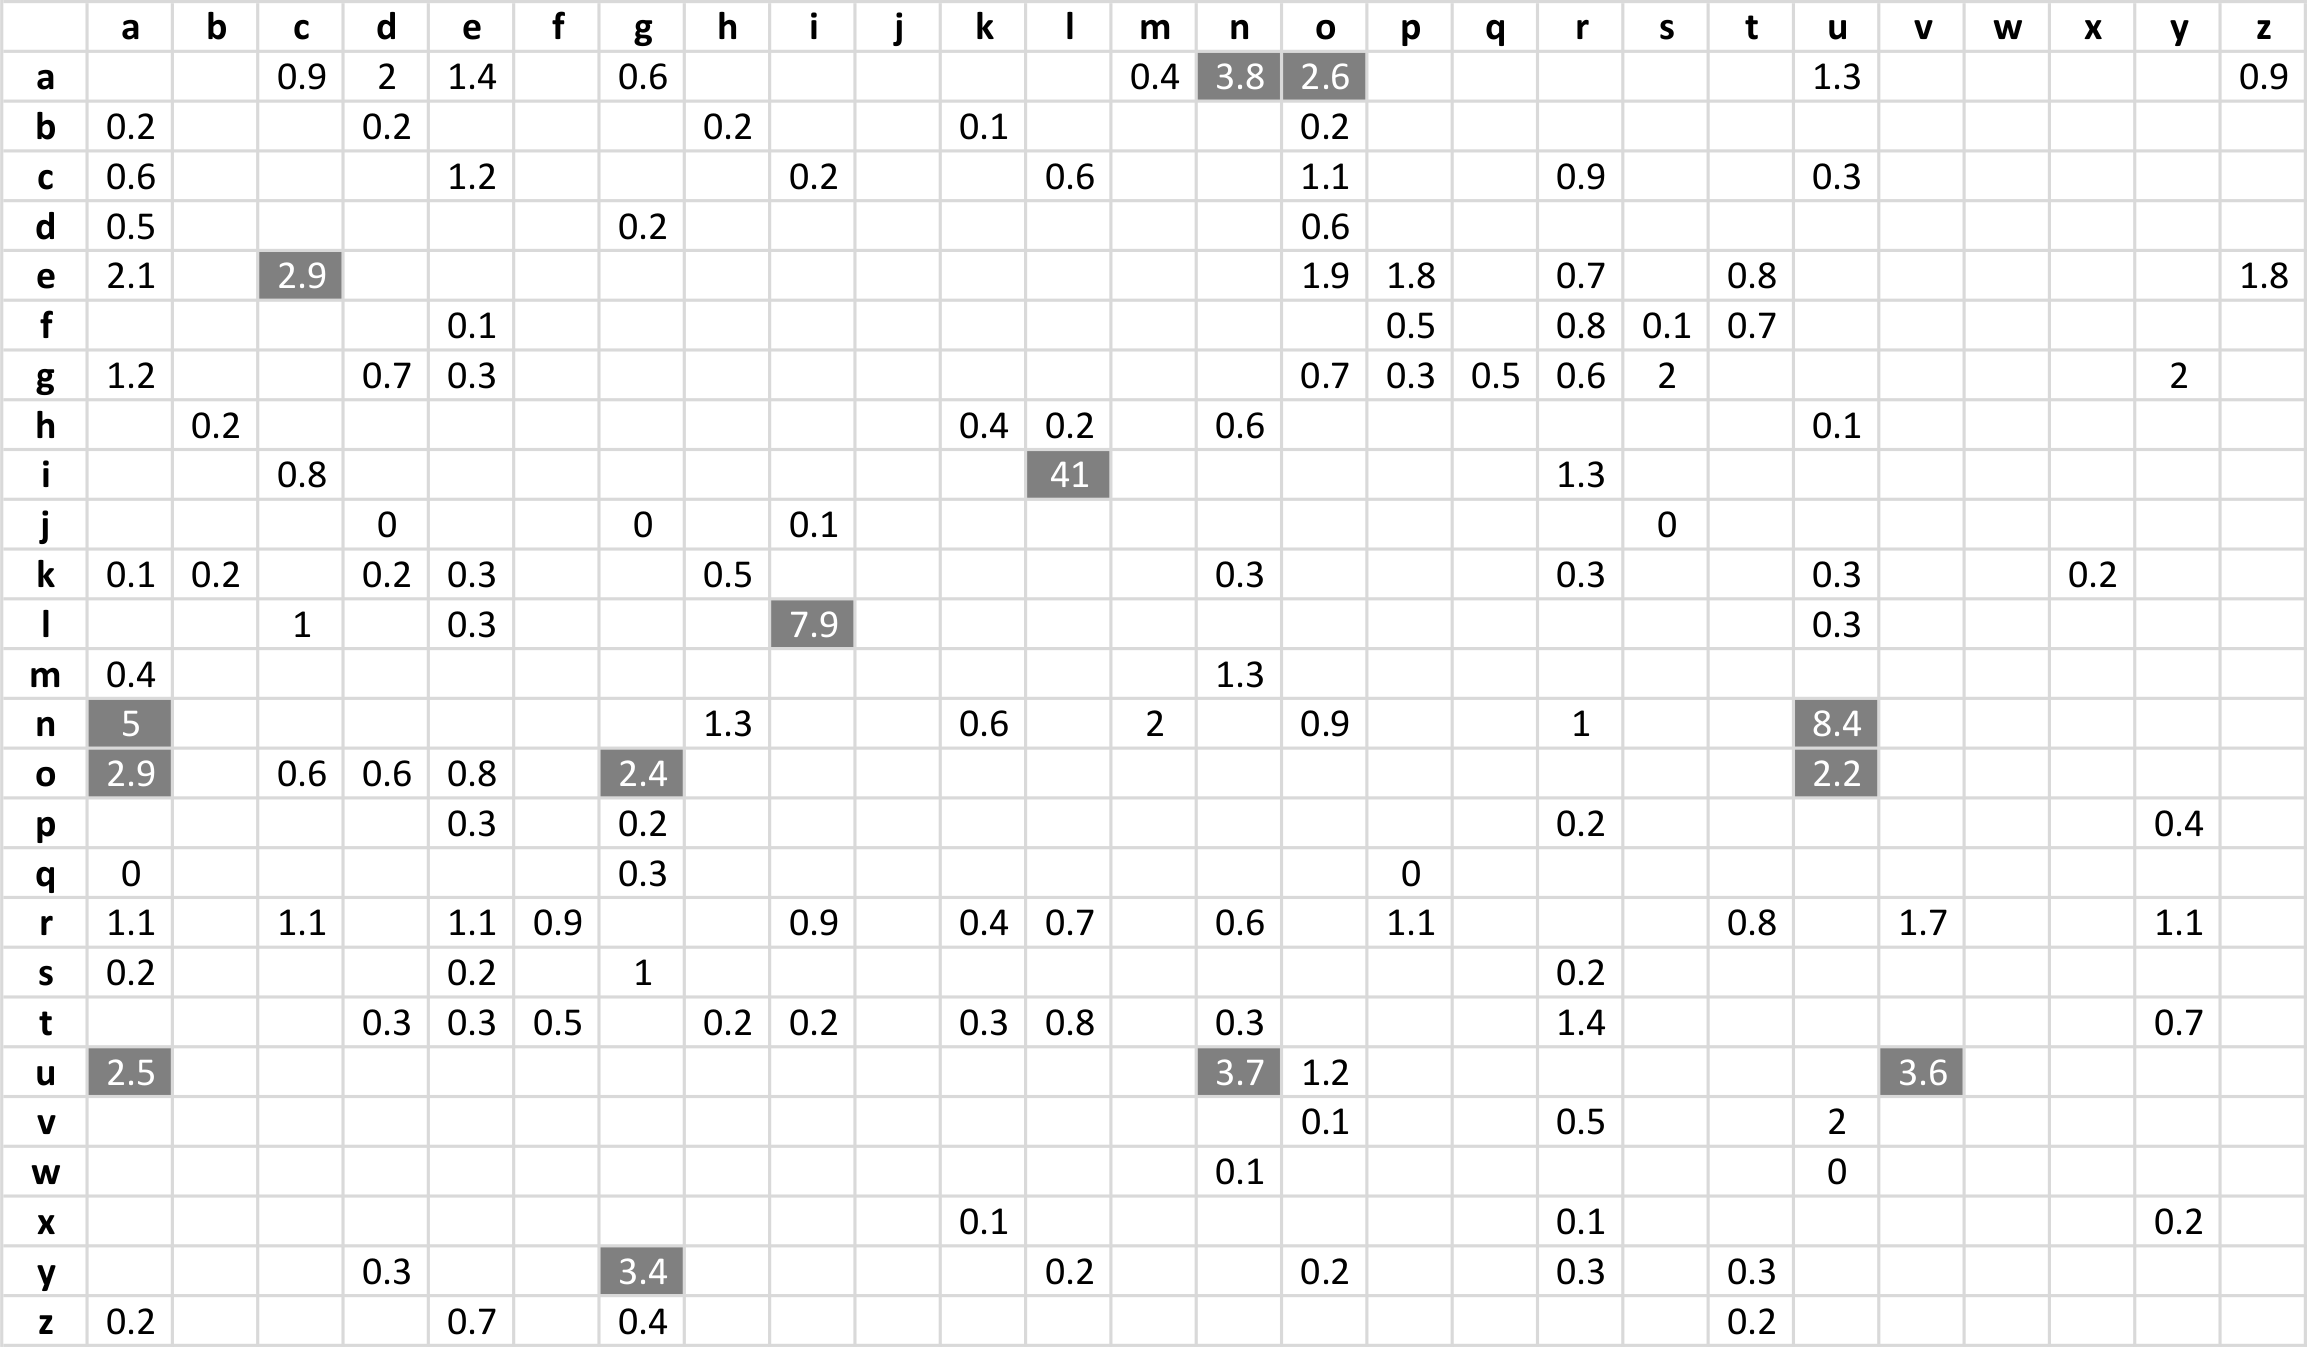
\includegraphics[width=135mm]{charmap.png}
\caption{Character misclassification map.  The correct label can be read from the left, and the
incorrect classification from the top.  The values have been scaled with the relative frequency of
the character in question.  The highest 10\% of values has been highlighted.}
\label{fig:charmisclassifications}
\end{figure}

% TODO: Explain the mystery of "q" with the fig:charmisclassifications map.

From this map it is also easy to recognize the most common pairs of characters to be misclassified.
By far the most common pair is "i" and "l".
% TODO: Explain why commonly "i" -> "l", but not so commonly vice versa; due to frequencies..?
This is understandable, considering the visual similarity of "i" and "l" as seen in Figure
\ref{fig:charpairs}; the leftmost instance of "i" looks in fact exactly like an instance of "l".
The second most common pair to be misclassified is "u" and "n", and the third most common pair is
"n" and "a".  The second "n" from the left demonstrates well the difficulty in discriminating them
from instances of "u", whereas the first two instances of "a" (with their open tops) could very well
be confused with an "n" or even a "u".  Such a visual comparison is a good reminder as to how
challenging the classification task at hand actually is, and helps appreciate the performance of the
algorithm where even the human observer may occasionally fail.

\begin{figure}[t]
\centering
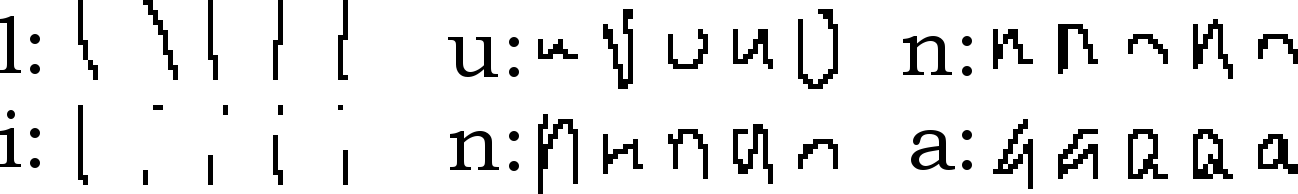
\includegraphics[width=100mm]{pairs.png}
\caption{The most commonly misclassified character pairs, by example.  Specimens have been randomly
selected from the correctly labelled data set.}
\label{fig:charpairs}
\end{figure}

\label{ref:datachallenge}

% TODO: Fill in X & Y below
The voluntary competition amongst other solutions to the same classification problem mentioned in
Section \ref{ref:datasetdescription} ended up favoring our solution.  The closest contender (at an
error rate of X\%, compared to our Y\%) was, interestingly, an implementation of kNN, which was
discussed as one of our early candidates in Section \ref{ref:knn}.  What made the solution
interesting was its simplicity - kNN is one of the simplest methods of machine learning, yet still
quite effective with suitable kinds of problems \cite{keller1985fuzzy}.

%\begin{itemize}
%\item k-fold cross validation: k=20, error rate 11\%
%\item k-fold cross validation: k=5, error rate 11.5\%
%\item One iteration with training set n=40000 and validation set n=2152 about 17 min with 2.1GHz Xeon (single thread)
%\item about 300MB of memory for training set n=42152
%\item Predicting one character: about 2 milliseconds
%
%\end{itemize}

% TODO: Re-enable this section..? Note that some are superficially covered in "Method Selection"

%\section{Quick comparison to other algorithms}
%
%\begin{itemize}
%\item kNN (+PCA/LDA)
%\item ...?
%\end{itemize}
%
%\cite{albanese12mlpy}

%============================================================

\bibliography{references}
\end{document}

